
\chapter{Sensor annex}

% [metre le détail des methodes ICA si pas assez de maths]

\section{CSP algorithm}

\subsection{CSP running time optimization}
\label{Sec:running_time_optimisation}

The optimization of the computation time does not change the neuroanatomical results presented, and therefore is not integrated in the "method" part, but still required a considerable amount of work.

My first implementation of the CSP algorithm took a whole day to compute for a single subject, which corresponds to a 15 days computation for our cohort. It was therefore crucial to find ways to greatly accelerate the calculations, which will then be reiterated at each commit of the pipeline as part of the continuous integration with Circle CI.

A great deal of research and engineering effort was then put into reducing the calculation time.

\paragraph{Classic software engineering techniques}

Classic software engineering techniques have been key to massively reduce computation times: factoring of all steps, use of tools such as the line-profiler — which allows to visualize the execution time of each line —  use of multi-processing. On the other hand, even if mathematically some operations are commutative, in practice, the choice of the order of the operations allows saving computation time: for example even if the operations (time crop, frequency filter) are commutative, it is better to start by cropping the data and then filtering, because the filtering operation is very expensive.

\paragraph{Dimensionality reduction}

Once all the software improvements have been made, we can also make improvements coming from machine learning techniques by using dimensionality reduction techniques: We can either select the type of channels, or use a PCA.

\begin{figure}[ht]
    \centering
    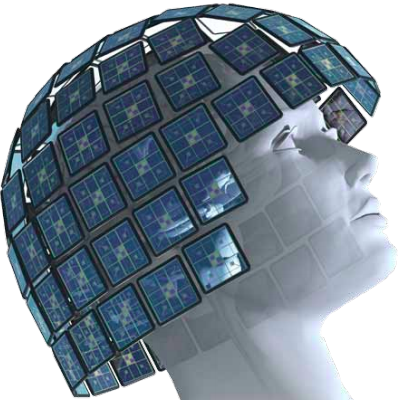
\includegraphics[width=5cm]{images_report/sensor/sensors_elekta.png}
    \caption[MEG Sensors]%
    {MEG Sensors [\href{https://www.elekta.com/dam/jcr:ed6d88e7-cd3e-478e-9c4a-3f89ef90ec92/Elekta-Neuromag-TRIUX-Brochure.pdf}{Elekta documentation}]}
    \label{sensors_elekta}
\end{figure}

\begin{itemize}
    \item Reduction of dimensionality by selection of the channel type: The MEG data comes from 102 sensors, which are distributed as shown in the figure \ref{sensors_elekta}. Each sensor consists of 2 gradiometers measuring the gradiometric field (Tesla/meter) in the direction tangent to the sensor plane, and a magnetometer measuring the electric field in the direction normal to the sensor plane. Magnetometers are robust to external noise, while magnetometers are more exposed. But magnetometers have two crucial advantages: 1. they record localized spatial information, which is perfectly suited to the CSP algorithm, which subsequently favors the interpretability of patterns from the CSP. 2. The magnetometers are half as numerous as the gradiometers.Thus, by selecting only the magnetometers, the number of channels is divided by three.  The CSP algorithm being limited by an SVD whose complexity in $\mathcal{O}(T n^2)$ evolves as a function of the square of the number $n$ of channels \cite{dhillonalan}, we thus accelerate the algorithm by a factor 9. (T is the number of time point, in our case bigger than the number of channels. The complexity of the SVD internal to the CSP is in the square of the minimum between $T$ and $n$).
    \item The following point applies only to data from a MEG, but not to EEGs. Indeed, EEGs have only one channel type. We can therefore reduce the dimensionality using a simple PCA.
\end{itemize}


\paragraph{Sampling}

The last way to accelerate the computation time is to use sampling, i.e. to reduce the sampling frequency. This is also called decimation. For example, $decim = 5$ consists in taking only one point on 5. But sampling can introduce numerical instabilities. Indeed, the CSP algorithm must start by estimating the covariance matrix of the signal. However, the estimation of a covariance matrix of dimension $n$ requires at least approximately $n$ points. With a sampling frequency of 100 Hz, over a time window of 0.5 seconds, we have 50 points. It is therefore necessary to reduce the dimensions to at most 50 or to use covariance regularization methods, presented in section \ref{CSP_regularization}.

[Nyquist]

\paragraph{CSP running time optimization results}

The choice of the order of commutativity, the reduction of the dimensionality and the resampling allow us today to obtain results in less than three hours with 8Cross validation for all subjects. These three techniques allow us to respectively accelerate by $2*10*5$ on our dataset while keeping similar performances in all points. It even seems that the PCA increases the numerical stability of the results.

% - Interaface avec le reste de la pipeline, openscience, reproductibilité
% - Anexes : Implémentation et choix d'architecte logiciel

% \subsection{Iterations levels}

% Choisir l'ordre des iterations n'a pas été une mince affaire, bien que ce soit ici plus un probleme d'ingénieurie que de la recherche pure.
% - contrasts
% - We iterate through subjects and sessions
% - If there are multiple runs, runs are concatenated into one session.

\subsection{CSP Regularization}
\label{CSP_regularization}
In order to regularize the estimation of the covariance matrix, many strategies exist, notably based on Riemannian geometry. But in our case, it is enough to use a regularization of diagonal elements of the covariance matrix, in order to obtain strictly positive eigenvalues. Thus, it is sufficient to replace the empirical estimate $C$ of the covariance matrix by :

\begin{equation}
    C' = C + \sum_k {\varepsilon_k \bar{\sigma_k}^2 I^{(k)}}\ ,
\end{equation}

with $k$, the index of the considered channel type, $\varepsilon_k$ the regularization coefficient, $\sigma_k$ the average standard deviation of the considered channel type, $I^{(k)}$ the matrix with 1 diagonal matrices containing ones at the positions corresponding to the channels contained in each channel group.

We used $\varepsilon_k = 0.1$.

% \subsection{CSP : Variance vs Second order moment}
% \subsection{CSP Solving}

\subsubsection{topographic map, right-hand rule}

\begin{figure}
    \centering
    \begin{subfigure}[b]{0.55\textwidth}
       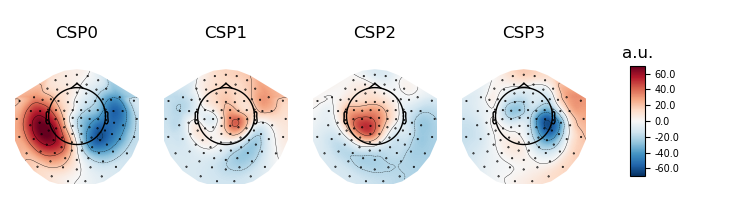
\includegraphics[width=1\linewidth]{images_report/sensor/csp_individual/sub_155_alpha.png}
       \caption{Example of CSP components (alpha band)}
       \label{fig:csp_component_alpha_band}
    \end{subfigure}
    
    \begin{subfigure}[b]{0.55\textwidth}
       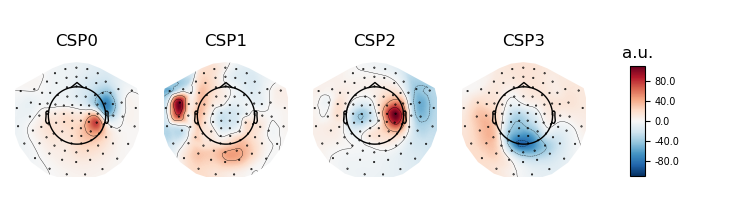
\includegraphics[width=1\linewidth]{images_report/sensor/csp_individual/sub_215_beta.png}
       \caption{Example of CSP components (beta band)}
       \label{fig:csp_component_beta_band}
    \end{subfigure}

    \caption[Example of CSP components from the alpha and beta band.]%
    {Example of CSP components from the alpha and beta band.}
    \label{example_csp_component}
\end{figure}

The visualization of CSP patterns makes it one of the most interpretable algorithms. But in the context of MEGs, one must keep in mind that the activations are done by magnetic dipole. Thus, in the CP0 of the figure, by using the right-hand rule, we deduce that the magnetic field enters inside the right ear.

\subsection{Mathematical subtleties}

\subsubsection{Why not aiming for the best classifier?}
Mathematically, we are not looking here to create the best classifier, and to optimize the ROC-AUC score, we are only looking to obtain unbiased scores that can be used later in the permutation test. This is why it is not a problem to optimize the execution time.

Moreover, in neuroscience, interpretability is much preferred to performance. And the CSP algorithm is ultra interpretable thanks to the visualization of patterns. Since our results are already significant with CSP, there is no need to struggle any further. The CSP algorithm is already one of the best compromise between interpretability and performance.


% \subsubsection{philosophie de pourquoi c'est ok de réduire un peu les performances, Pourquoi ne pas se battre pour les performances avec les CSP.}

% By thinking more about it, It feels to me that this group cross validation is not even necessary at all for mathematical rigor. Because here we just want to construct a statistic for each frequency bin. Here our statistic is the size of the cluster after thresholding the ROC-AUC score coming from a usual cross validation. But our statistic could really be anything. The permutation test is just here to confirm that "There is a difference", whatever the difference is. So it's perfectly valid to use any metric : accuracy is as legitimate as ROC-AUC and our cross validation is as legitimate as a group cross validation.
% Another way to say it is that : we do not want to test the generalization ability of our classifier between different runs. We just want to say : Our classifier proves a difference exists between the two conditions.
% So I think no need to worry because no need for group cross-validation.


% \subsubsection{Possiblité de mettre un des frequences et des crop non uniformes}

\subsubsection{Choosing the t-value threshold}

The fact that you can choose the size of the clusters simply by adjusting the threshold of the t-value is disturbing at first sight. But in reality, it is a good sign. We only tested two different t-values (0.01 and 0.05) and the fact that we get two different cluster sizes simply means that our 0.05 cluster has a significant difference as well as our 0.01 cluster, which is also significant. One does not exclude the other.

Choosing a t-value threshold of $0.01$ we obtain the figure \ref{permutation_statistics_results}, with a cluster having a p-value of $10^{-3.6}$. I chose this restrictive threshold of 0.01 for my final image in order to limit the area of my cluster and to limit it to the most significant areas. But it is possible by choosing a threshold of $0.05$ to obtain a figure with a cluster going through the whole alpha band from 0 to 5 seconds.

However, the obtained cluster has no physical reality and could be extended to the whole image if we had more subjects. We must therefore take a cluster of reasonable size in order to maximize the signal-to-noise ratio when moving to the analysis of sources.


\subsubsection{Difficulties concerning the calculation of an average of the CSP components}
\label{section:csp_average_difficulty}

We have thought about the feasibility of calculating the averages of the CSP components in order to obtain "average" components shared by all subjects. But some difficulties make these averages unfeasible:
\begin{itemize}
    \item Although the CSP components are ordered by decreasing eigenvalue, there is a great risk of mixing CSP components across different anatomical regions for different subjects. To mitigate this risk, one would have to do a CSP decomposition for each brain area, which would complicate the operation.
    \item Using the same CSP components for everyone would necessarily lower the decoding results. Considering that our subjects probably use different memorization strategies, these different strategies would be "mixed" in a group decoding, and would harm the interpretability.
\end{itemize}

\section{Cluster permutations statistics algorithm}

\subsection{t-values calculation}

This test rejects the null hypothesis that the mean of a population of independent observations is equal to a value $M$.

\paragraph{Hypothesis}

The t-test is a parametric test that assumes the Gaussianity of the underlying values. This assumption of Gaussianity is not always true for data from brain imaging because of the many preliminary filters. But in our case, we compute t-values from the difference between the ROC-AUC score and the average chance level, which allows us to restore the Gaussianity assumption.

\paragraph{Intuition}

The calculation of p-values is done for each time frequency bin independently.

We consider the list of differences $(X_i)_{i \in [\text{Nb Subjects}]}$ for all subjects between the ROC-AUC and the chance level $M=0.5$ for a bin of temporal frequency. We obtain the set of differences between the ROC-AUC and the chance level. A normal distribution of these differences is made. If the normal distribution is sufficiently to the right of 0, then we reject the null hypothesis.

\paragraph{Algorithm}

We want to compare the mean $\mu$ of a population with a normal distribution and an unknown standard deviation $\sigma$ to $0$. To do this, we compute the empirical mean $\overline{x} = \frac{1}{n}\sum_{i=1}^{n}x_i$ and the unbiased estimator $S^{\ast ^2}_n$ of variance $\sigma^2$

$S^{\ast ^2}_n = \frac{1}{n-1}\sum\limits_{i=1}^n (X_i - \overline X_n )^2$.

According to the null hypothesis, the sampling distribution of this mean is also normally distributed with a standard deviation $\frac{\sigma}{\sqrt{n}}$.

The test statistic:

$ Z = \sqrt{n}\frac{\overline{X} - \mu_0}{S^{\ast}_n}$
then follows a Student's law of $n-1$ degrees of freedom under the null hypothesis.

We choose a risk $\alpha$, generally $0.05$ or $0.01$ and we calculate the realization of the test statistic :

$z = \sqrt{n}\frac{\overline{x}_n - \mu_0}{s^{\ast}_n},$ where $s^{\ast}_n =\sqrt{\frac{1}{n-1}\sum\limits_{i=1}^n (x_i - \overline x_n )^2} $

\subsection{Choosing the number of time-frequency bin}

Choosing the number of Bin is somewhat arbitrary. One just has to respect some conditions such as Nyquist, plus the fact of having enough points to estimate the covariance matrix. But here, it is not serious to choose arbitrary the number of points, since the result of the sensor space is only used to increase the signal-to-noise ratio when going into the source space.

\chapter{Source annex}


\section{Dynamic statistical parametric mapping (dSPM)}

\paragraph{Method}

Dynamic statistical parametric mapping allows to obtain a three-dimensional image of the sources by taking into account the activation of the baseline. For each three-dimensional point, a normalization by the noise variance is performed. The resulting image gives the activation map, made of positive intensities only.

\paragraph{Choice of covariance matrix}

In order to calculate the source estimate by dSPM, we need to choose a covariance matrix, in order to know the covariance of the signal not carrying the information. The choice of the covariance matrix is therefore not a mathematical problem, but a choice that follows from our experimental paradigm. We must answer the question: what constitutes noise? Here are the two main choices of covariance matrix:
\begin{itemize}
    \item Use the empty room covariance. This is the covariance matrix associated with sensor noise when there is no one in the room. This is the default choice in the MNE-BIDS-Pipeline.
    \item Use the pre-stimulus covariance. Indeed, before the cue, the participant does not yet know the duration of the cue. This is the method we recommend.
\end{itemize}

% Subtilités mathématiques :  commutativité Log + moyenne

\section{Boundary Element Model (BEM)}

\begin{figure}[ht]
    \centering
    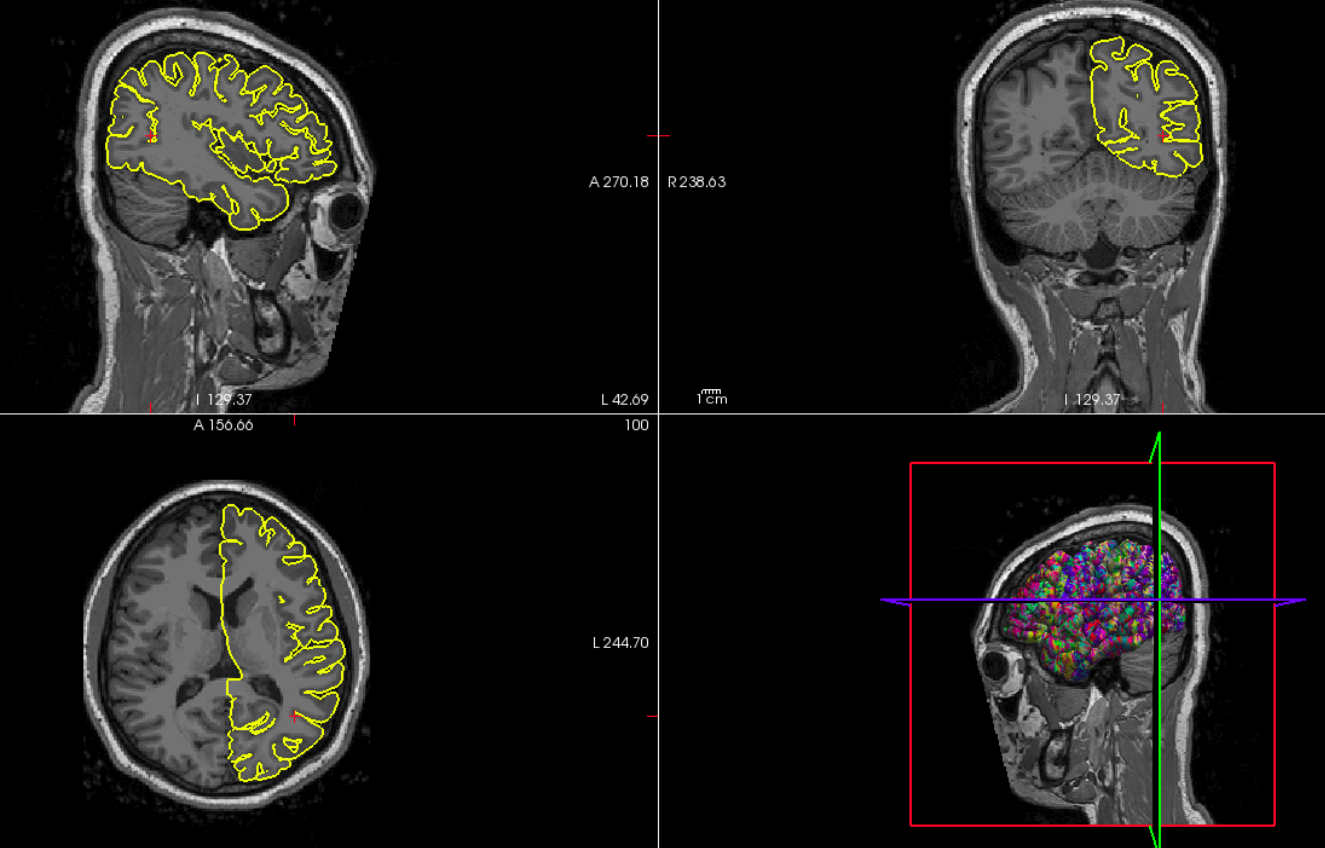
\includegraphics[width=15cm]{images_report/source/BEM_model_freeview_cropped.png}
    \caption[BEM model used for one of our anonymized subjects.]%
    {BEM model used for one of our anonymized subjects.}
    \label{BEM_model_freeview_cropped}
\end{figure}


Figure \ref{BEM_model_freeview_cropped} presents the boundary element model used to model one of our subject's heads. Our participants were recorded by MRI before their MEG recording in order to obtain T1 anatomical images. These T1 images are used to create a 3D model of the brain and to model each area of the brain with different electromagnetic conductivity. This model is then used to calculate the inverse operator to find the location in the brain of the electromagnetic sources from the MEG recording.

We can see on the figure \ref{BEM_model_freeview_cropped} that the face of the person has been cut in order to anonymize the data.  We can see on the figure the result of the segmentation between the white matter and the gray matter. The results of the algorithm, although satisfactory, are not perfect. But this is of little importance because MEG is a relatively robust technique with respect to the imperfections of electromagnetic conductivity modeling. For example, for EEG we use generally 3 layers (inner skull, outer skull, and skin) while for MEG 1 layer (inner skull) is enough: The MEG is said to be "transparent".


